%% CAPITOLO 2
\clearpage
\chapter{Analisi tecnica}\label{ch:technical-analysis}
In questo capitolo si effettua una analisi tecnica, relativa alle tecnologie adoperate, per ottenere un'ampia panoramica sul loro utilizzo e sulle loro funzionalità.

\section{Il framework: Spark}\label{sec:spark}

La tecnologia fondamentale che costituisce il fulcro del progetto è \href{https://spark.apache.org/docs/latest/rdd-programming-guide.html}{Spark}.
I programmi Spark richiedono l'impiego di 5 entità:
\begin{itemize}
    \item un driver program;
    \item un cluster manager;
    \item molteplici worker;
    \item degli executor;
    \item dei task.
\end{itemize}
Un \textit{driver program} è una applicazione che usa Spark come libreria e costituisce il punto d'ingresso di tutto il sistema;
volendo, costituisce il \textit{main} del programma.
Per connettersi al \textit{cluster manager}, e quindi agli eventuali cluster, è necessario inizializzare uno \texttt{SparkContext} che stabilisce la connessione.
Il \textit{cluster manager} inizializza dei nodi \textit{worker} che forniscono memoria e storage all'applicazione Spark.
Su ogni \textit{worker}, vengono create delle JVM (\textit{Java Virtual Machine}) che costituiscono gli \textit{executor}.
Ogni \textit{executor} è in grado di eseguire molteplici \textit{task} assegnati dal \textit{cluster manager}.
Un programma Spark è in grado di lanciare molteplici \textbf{job}, dove un \textit{job} rappresenta un insieme di computazioni necessarie per restituire un risultato al \textit{driver program}.
Un \textit{job} può essere suddiviso in \textbf{stage}: nello specifico, Spark crea un \textit{directed acyclic graph} (DAG) di \textit{stage}, e suddivide ogni \textit{stage} in molteplici \textbf{task}~\cite{big-data-spark}.
I task possono essere visti come la più piccola unità di lavoro eseguibile dagli executor.
Una volta ottenuto il risultato dei task, gli \textit{executor} possono inoltrarlo al \textit{driver program}.
La figura~\ref{fig:spark-application} è una rappresentazione della comunicazione tra queste entità.
\begin{figure}
    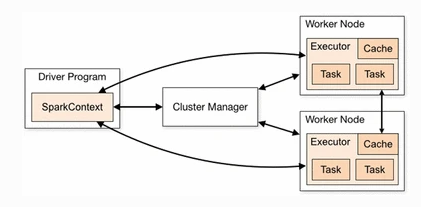
\includegraphics[width=\textwidth]{img/spark-application.png}
    \centering
    \caption{Funzionamento di un programma Spark.}
    \label{fig:spark-application}
\end{figure}

\subsection{Storia}\label{subsec:spark-history}

Il progetto Spark è nato nel 2009 alla \textit{Berkeley’s AMPLab, University of California} per poi essere donato alla \textit{Apache Software Foundation} nel 2013~\cite{big-data-spark}.
Il progetto consiste di diverse componenti principali, tra cui \textit{Spark SQL}, \textit{Spark MLlib} per il machine learning, \textit{GraphX} e \textit{Spark Streaming}.
Storicamente, Spark ha introdotto un'astrazione per modellare algoritmi e processi con migliori prestazioni: i \textbf{Resilient Distributed Dataset} (\textit{RDD}).
Un RDD è una collezione di record partizionati e \textit{read-only};
rappresenta una struttura dati parallela e \textit{fault-tolerant},, il cui partizionamento e contenuto può essere manipolato attraverso una serie di operazioni~\cite{big-data-spark}.
Tutte le componenti di Spark sfruttano la astrazione degli RDD;
tuttavia, il progetto Spark è in continua evoluzione.
Ciò ha portato a diverse feature che hanno sostituito gli RDD:
tra queste, vi è l'introduzione dei \textbf{DataFrame}, facenti parte del modulo \textit{Spark SQL}.
Un \textit{DataFrame} è concettualmente equivalente ad una tabella di un database relazionale, ma distribuita e con trasformazioni ottimizzate.
La feature più importante rispetto agli RDD è quella dei dati organizzati in colonne.

Un altro miglioramento è stato introdotto nella versione Spark 1.6 con i \textit{Dataset}.
In particolare, l'obiettivo dei \textit{Dataset} è quello di unire i vantaggi degli RDD e dell'ottimizzazione dell'\textit{execution engine} di \textit{Spark SQL}.

\subsection{Datasets}\label{subsec:datasets}

\textit{Spark} permette di eseguire operazioni parallele su molteplici cluster remoti.
Il vantaggio che questa libreria porta è quello di scrivere codice parallelo con una sintassi sequenziale, effettuando operazioni tipizzate su \href{https://spark.apache.org/docs/latest/api/scala/org/apache/spark/sql/Dataset.html}{Dataset} distribuiti.
Un \textit{Dataset} è una \texttt{collection} fortemente tipizzata di oggetti che possono essere trasformati in parallelo e sono mappati ad uno schema relazionale.
Ogni \textit{Dataset} ha anche una vista non tipizzata chiamata \textbf{DataFrame}, che consiste in un \texttt{Dataset} di \href{https://spark.apache.org/docs/latest/api/scala/org/apache/spark/sql/Row.html}{Row};
una \texttt{Row} rappresenta una riga di output di un operatore relazionale.

I dati sono distribuiti sui cluster, e \textit{Spark} rende completamente trasparente il partizionamento agli sviluppatori.
In particolare, questo paradigma distingue le operazioni eseguibili sui \textit{Dataset} in \textbf{Azioni} e \textbf{Trasformazioni}.
Le trasformazioni sono operazioni che producono nuovi \textit{Dataset} come output;
tra le trasformazioni, alcune delle più comuni sono:
\begin{itemize}
    \item \textit{map} - applica una trasformazione a tutti gli elementi del \textit{Dataset}.
    \item \textit{filter} - permette l'applicazione di un filtro sugli elementi del \textit{Dataset}, rimuovendo quelli che non rispettano il predicato passato come argomento.
    \item \textit{select} - esegue una espressione-colonna sul \textit{Dataset}, ritornandone uno con le colonne specificate nell'espressione.
    \item \textit{union} - unisce gli elementi di due \textit{Dataset}.
    \item \textit{join} - esegue l'operazione di \textit{join} tra due \textit{Dataset}.
    Tale trasformazione permette di specificare una \textit{join expression}, che determina i campi da utilizzare per l'operazione.
    Inoltre, permette di definire il tipo di \textit{join} della trasformazione;
    i tipi di \textit{join} sono elencati e descritti nella sezione~\ref{subsec:join}.
    \item \textit{withColumn} - aggiunge una colonna al \textit{Dataset} con una \textit{column-expression}.
    \item \textit{drop} - rimuove dal \textit{Dataset} la colonna specificata.
\end{itemize}
Invece, le azioni sono operazioni che provocano delle computazioni le quali ritornano dei risultati.
Nello specifico, richiedono di reperire in locale il contenuto distribuito dei \textit{Dataset}.
Alcune azioni sono:
\begin{itemize}
    \item \textit{collect} - ritorna un array con il contenuto del \textit{Dataset}.
    \item \textit{count} - ritorna il numero di elementi del \textit{Dataset}.
    \item \textit{foreach} - esegue una funzione su ogni elemento del \textit{Dataset}.
    \item \textit{reduce} - riduce il \textit{Dataset} applicando una funzione binaria.
    \item \textit{show} - mostra su standard output (\texttt{stdout}) i primi \textit{n} elementi del \textit{Dataset}.
    \item \textit{write} - scrive in output il \textit{Dataset} con il formato e percorso specificati.
\end{itemize}
Questa distinzione è necessaria in quanto il paradigma di \textit{Spark} costruisce un \textbf{piano logico} che rappresenta le computazioni necessarie per restituire i dati di un \textit{Dataset}.
Infatti, i \textit{Dataset} hanno un comportamento \textit{lazy}: le computazioni vengono eseguite in parallelo a \textit{runtime} solamente alla chiamata di un'azione (figura~\ref{fig:transformations-actions}).
Quando viene invocata un'azione, l'ottimizzatore di \textit{Spark} ottimizza il piano logico e produce un \textbf{piano fisico} per eseguire le query efficientemente in maniera parallela e distribuita~\cite{spark-dataset}.
Questa distinzione permette di rendere Spark estremamente dichiarativo:
le sole trasformazioni permettono di gestire enormi moli di dati senza che queste vengano effettivamente eseguite a runtime nel momento in cui si dichiarano.
\begin{figure}[H]
    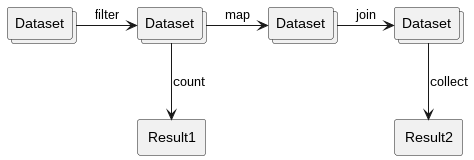
\includegraphics[width=\textwidth]{img/transformations-actions.png}
    \centering
    \caption{Esempio di esecuzione di trasformazioni e azioni su \textit{Dataset}.}
    \label{fig:transformations-actions}
\end{figure}
In più, la gestione dei tipi di dati dei \textit{Dataset} permette di individuare eventuali errori nel piano logico senza dover aspettare l'effettiva esecuzione di quello fisico;
ad esempio, l'invocazione di una \textit{select} su un determinato campo può specificare che tale campo non esiste nel \textit{Dataset};
oppure, una funzione di aggregazione per somma può restituire un errore logico se viene effettuata su una colonna di stringhe.

Inoltre, è possibile salvare in memoria il contenuto di un \textit{Dataset} grazie al metodo \texttt{Dataset.cache()}.
Ciò può essere estremamente utile nel caso in cui vengano effettuate più computazioni su uno stesso \textit{Dataset}:
mantenerne il contenuto in memoria permette di risparmiare tempo d'esecuzione del \textit{job} per eseguire ulteriori \textit{job} sullo stesso cluster.
In aggiunta, è considerata come una operazione \textit{lazy}, cioè che le informazioni del \textit{Dataset} non vengono effettivamente rese persistenti fino all'invocazione di un'azione.

\subsection{L'operazione di \textit{join}}\label{subsec:join}
La trasformazione di \textit{join} è una delle più importanti poichè permette di combinare informazioni contenute in diversi \textit{Dataset} con una specifica \textit{join condition}.
Quando si applicano queste trasformazioni bisogna tener conto delle moli di dati che vengono \textbf{combinati in maniera distribuita}:
spesso si può incorrere in problemi di prestazioni dovuti ad un utilizzo non corretto delle trasformazioni di \textit{join}.
Ad ogni modo, le trasformazioni di \textit{join} sono ottimizzate da Spark di default, ma questo non significa che non vada prestata attenzione nel loro utilizzo~\cite{spark-join}.
Spark supporta tutti i principali tipi di \textit{join} di SQL;
di seguito vengono elencati e brevemente descritti prendendo come riferimento i \textit{DataFrame}:
\begin{itemize}
    \item \textbf{Inner Join} (figura~\ref{fig:inner-join}) - Corrisponde alla \textit{join} di default.
    Viene utilizzata per combinare due \textit{DataFrame} considerando delle colonne chiave.
    Laddove non vi sia corrispondenza tra le chiavi, le righe vengono rimosse da entrambi i \textit{DataFrame}.
    Corrisponde all'individuazione dell'intersezione di due insiemi di dati, dove l'intersezione coincide con l'uguaglianza di determinati campi.
    \begin{figure}[H]
        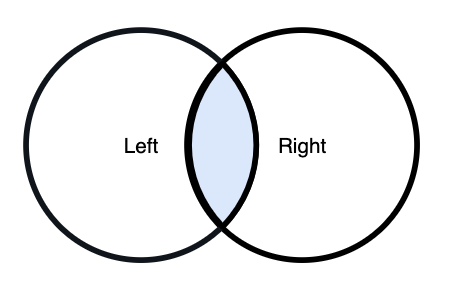
\includegraphics[width=.5\textwidth]{img/inner-join.png}
        \centering
        \caption{Esempio figurato di una \textit{inner join} tra due \textit{Dataset}: colonne di entrambi e righe che soddisfano la \textit{join condition}.}
        \label{fig:inner-join}
    \end{figure}
    \item \textbf{Full Outer Join} (figura~\ref{fig:outer-join}) - Restituisce le righe di entrambi i \textit{DataFrame}, lasciando il valore \texttt{null} nelle rispettive colonne quando le chiavi non corrispondono.
    \begin{figure}[H]
        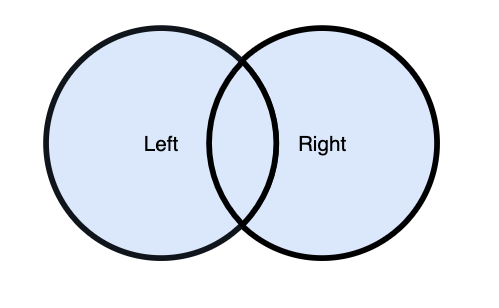
\includegraphics[width=.5\textwidth]{img/outer-join.png}
        \centering
        \caption{Esempio figurato di una \textit{full outer join} tra due \textit{Dataset}: righe e colonne di entrambi.}
        \label{fig:outer-join}
    \end{figure}
    \item \textbf{Left Outer Join} (figura~\ref{fig:left-join}) - Restituisce tutte le righe del \textit{DataFrame} di sinistra, a prescindere dalla corrispondenza delle chiavi.
    Laddove non vi sia corrispondenza tra le chiavi, le colonne del \textit{DataFrame} di destra vengono valorizzate con \texttt{null}.
    Viene utilizzata quando non si vuole alterare la dimensione di un \textit{DataFrame}, bensì si vuole arricchire di informazioni se presenti all'interno di un altro (quello di destra).
    \begin{figure}[H]
        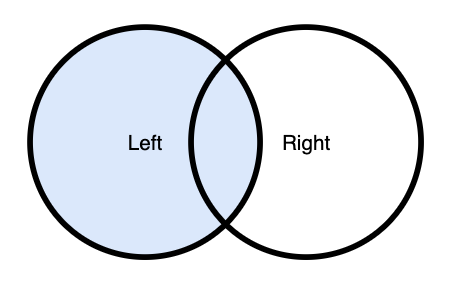
\includegraphics[width=.5\textwidth]{img/left-join.png}
        \centering
        \caption{Esempio figurato di una \textit{left outer join} tra due \textit{Dataset}: colonne di entrambi, righe di quello di sinistra.}
        \label{fig:left-join}
    \end{figure}
    \item \textbf{Right Outer Join} (figura~\ref{fig:right-join}) - Corrisponde al contrario della \textit{left outer join}.
    Restituisce tutte le righe del \textit{DataFrame} di destra, valorizzando con \texttt{null} le colonne di quello di sinistra laddove le chiavi non corrispondano.
    Equivale ad effettuare una \textit{left outer join} invertendo i \textit{DataFrame}, ma viene comunque messa a disposizione per comodità.
    \begin{figure}[H]
        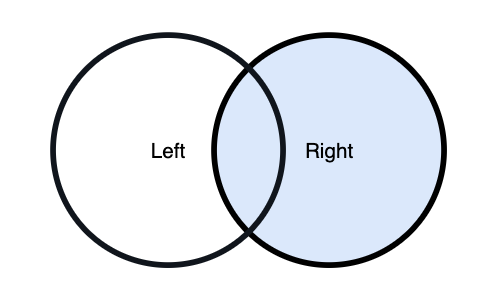
\includegraphics[width=.5\textwidth]{img/right-join.png}
        \centering
        \caption{Esempio figurato di una \textit{right outer join} tra due \textit{Dataset}: colonne di entrambi, righe di quello di destra.}
        \label{fig:right-join}
    \end{figure}
    \item \textbf{Left Semi Join} (figura~\ref{fig:left-semi-join}) - Equivale alla \textit{inner join}, tuttavia ignora le colonne del \textit{DataFrame} di destra.
    Più semplicemente, questa \textit{join} restituisce le righe del \textit{DataFrame} di sinistra quando si ha una corrispondenza delle chiavi.
    Corrisponde ad una \textit{inner join} seguita da una \textit{select} dei campi del \textit{DataFrame} di sinistra.
    \begin{figure}[H]
        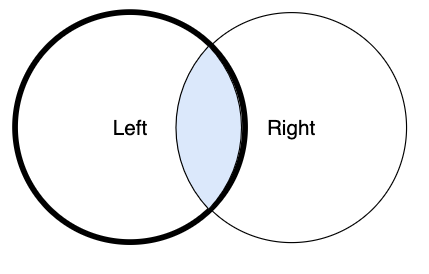
\includegraphics[width=.5\textwidth]{img/left-semi-join.png}
        \centering
        \caption{Esempio figurato di una \textit{left semi join} tra due \textit{Dataset}: colonne di quello di sinistra, righe che soddisfano la \textit{join condition}.}
        \label{fig:left-semi-join}
    \end{figure}
    \item \textbf{Left Anti Join} (figura~\ref{fig:left-anti-join}) - Corrisponde all'opposto della \textit{left semi join}.
    Restituisce le righe del \textit{DataFrame} di sinistra che non hanno una corrispondenza con quello di destra.
    \begin{figure}[H]
        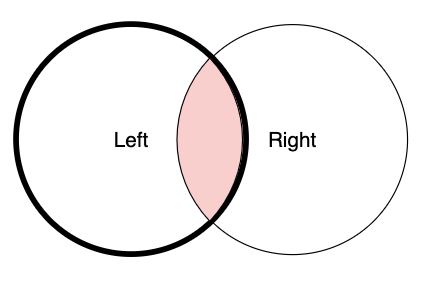
\includegraphics[width=.5\textwidth]{img/left-anti-join.png}
        \centering
        \caption{Esempio figurato di una \textit{left anti join} tra due \textit{Dataset}: colonne di quello di sinistra, righe che non soddisfano la \textit{join condition}.}
        \label{fig:left-anti-join}
    \end{figure}
\end{itemize}

\section{Il linguaggio: Scala}\label{sec:scala}

Il linguaggio di implementazione del progetto è \href{https://www.scala-lang.org/}{Scala2}.
La scelta del linguaggio è dovuta ad una dipendenza di Spark.
Le API dei moduli di Spark sono disponibili per diversi linguaggi;
tra i più utilizzati si trovano \textit{Python} e \textit{Scala}.
Inizialmente, i progetti Spark in Prometeia utilizzavano \textit{Python} come linguaggio d'implementazione.
Tuttavia, si è notato che un medesimo programma scritto in \textit{Scala} presentava prestazioni nettamente migliori, quindi si è scelto di passare a tale linguaggio.
Questa differenza di prestazioni è dovuta all'architettura stessa di Spark descritta nella sezione~\ref{sec:spark}.
Nello specifico, i nodi \textit{worker} istanziano una \textbf{Java Virtual Machine} su cui eseguire i vari task di Spark.
Quindi, quando devono eseguire un piano fisico relativo ad un \textit{Dataset} di oggetti \textit{Python}, è necessario convertire tali oggetti in \textit{Java}.
Questo passaggio invece non è necessario quando i \textit{Dataset} sono implementati in \textit{Scala} per via dell'interoperabilità con \textit{Java}.
Di conseguenza, è stato scelto di implementare i nuovi progetti Spark in \textit{Scala}.

In più, \textit{Scala} porta con sè ulteriori vantaggi, tra i quali:
\begin{itemize}
    \item Scalabilità - Anche il nome stesso suggerisce uno dei grandi vantaggi del linguaggio.
    Infatti, \textit{Scala} è una abbreviazione di \textbf{Scalable Language}, stando a indicare come questi sia utilizzabile per costruire sistemi scalabili, anche di grandi dimensioni.
    \item Supporto degli ambienti di sviluppo - Diversi ambienti di sviluppo supportano questo linguaggio.
    In particolare, l'IDE (\textit{Integrated Development Environment}) \textit{IntelliJ Idea} fornisce una serie di funzionalità che migliorano l'esperienza di sviluppo;
    ad esempio, una chiara \textit{syntax highlighting} e un supporto per la \textit{type inference} che permette di intercettare errori a \textit{compile time}.
    \item Sintassi semplificata - É un linguaggio più conciso rispetto a \textit{Java};
    infatti, spesso molteplici righe di codice \textit{Java} possono essere riassunte in una sola in \textit{Scala}.
    Basti pensare che tutte le operazioni degli \texttt{Stream} in \textit{Java} sono invocabili da una qualsiasi \textit{collection} di \textit{Scala}.
    \item Linguaggio funzionale - \textit{Scala} è un linguaggio che supporta l'\textbf{higher-order}.
    Ciò significa che le funzioni possono essere passate come argomenti ad altre funzioni e utilizzate come valori.
    Questa caratteristica può migliorare la qualità del codice prodotto dagli sviluppatori, così come può facilitare la scrittura di algoritmi e procedure.
    \item Interoperabilità con Java - Come sopra anticipato è molto facile far cooperare codice \textit{Java} e \textit{Scala}.
    Questo può essere d'aiuto nel caso di dipendenze da librerie o da altre componenti sviluppate in precedenza che diventano quindi riutilizzabili senza dover essere riadattate.
    \item Pattern Matching - Un costrutto molto utile che può essere visto come lo \texttt{switch} di \textit{Java} più potente.
    Può essere utilizzato per controllare il contenuto di una variabile, il tipo dinamico di un'istanza a \textit{runtime}, iterare liste e molto altro.
\end{itemize}

\section{Il cloud: Amazon Web Services}\label{sec:aws}

L’\textit{Infrastructure as a Service} (\textit{IaaS}) è una tipologia di \textit{Cloud Computing} basato sul consumo, come servizio, di risorse hardware.
Server virtuali, potenza di calcolo, storage, reti vengono messi a disposizione per essere utilizzati senza necessariamente dover affrontare costi di acquisto dell'hardware stesso.
In questo modo, chi adopera dell'infrastruttura ottiene il totale controllo delle risorse a sua disposizione.
Uno dei vantaggi maggiori rispetto all'acquisto diretto delle risorse è quello della manutenzione:
chi utilizza l’infrastruttura \textit{in cloud} non si deve preoccupare di fare manutenzione o rinnovare l’hardware;
si limita semplicemente ad utilizzare un servizio scalabile e affidabile senza preoccuparsi dei meccanismi di gestione interna.

Invece, il \textit{Platform as a Service} (\textit{PaaS}) rappresenta una tipologia di servizio fornito del tutto differente, anche se per diversi aspetti simile alle \textit{IaaS}.
Ad essere fornito come servizio, in questo caso, non è solo l'hardware, ma anche la piattaforma che permette di usufruire di un insieme di funzionalità le quali forniscono storage, reti, macchine virtuali, deployment, bilanciamento del carico (\textit{load balancing}) e altro ancora.
A differenza delle \textit{IaaS}, il meccanismo di queste funzionalità viene spesso oscurato: nelle \textit{IaaS} si ha pieno controllo delle funzionalità a disposizione, mentre nelle \textit{PaaS} no.
Il vantaggio per l'utente è quello di concentrarsi solo ed esclusivamente sullo sviluppo delle applicazioni, e non perdersi nell'analisi di problematiche legate all'ambiente in cui queste devono essere distribuite, ottenendo, contestualmente dalla piattaforma, la scalabilità e  l'affidabilità necessaria.
Inoltre, come per le \textit{IaaS}, l'utente non deve preoccuparsi di aggiornare i sistemi operativi:
viene tutto gestito dinamicamente e in modo del tutto automatico dalla piattaforma.
Se in determinati periodi si dovessero verificare carichi di picco, la piattaforma deve essere in grado di adeguare la propria struttura per rispondere alle nuove esigenze, anche se temporanee.

Tra le diverse tecnologie di \textit{Cloud Computing}, Prometeia fa anche uso di \textit{Amazon Web Services} (AWS) per la realizzazione di sistemi e servizi con supporto in \textit{cloud}.
Tra i diversi servizi che AWS mette a disposizione, durante il tirocinio sono stati utilizzati i seguenti:
\begin{itemize}
    \item \textbf{S3} - \textit{Amazon Simple Storage Service} è un servizio di archiviazione di risorse.
    Offre scalabilità, disponibilità dei dati, sicurezza e prestazioni all'avanguardia nel settore.
    I clienti di tutte le entità e settori possono archiviare e proteggere qualsiasi quantità di dati per qualsiasi caso d'uso, come \textit{data lake}, applicazioni native per il cloud e applicativi \textit{mobile}.
    Con classi di archiviazione convenienti e funzionalità di gestione di facile utilizzo, è possibile ottimizzare i costi, organizzare i dati e configurare controlli di accesso ottimali per soddisfare specifici requisiti aziendali, organizzativi e di conformità~\cite{aws-s3}.
    \item \textbf{Glue} - \textit{AWS Glue} è un servizio di integrazione dei dati serverless che facilita la scoperta, la preparazione, lo spostamento e l'integrazione dei dati da più origini per l'analisi e lo sviluppo di applicazioni~\cite{aws-glue}.
    \textit{AWS Glue} può eseguire i processi di estrazione, trasformazione e caricamento (ETL) non appena arrivano nuovi dati.
    Ad esempio, si può configurare per eseguire il processo ETL non appena i nuovi dati diventano disponibili su Amazon S3 (vedi figura~\ref{fig:event-based-etl-on-glue}).
    \item \textbf{DynamoDB} - \textit{Amazon DynamoDB} è un database NoSQL serverless e completamente gestito, progettato per eseguire applicazioni ad alte prestazioni su qualsiasi scala.
    Offre sicurezza integrata, backup continui, repliche multi-regione automatizzate, caching interno alla memoria e strumenti di importazione ed esportazione dei dati~\cite{aws-dynamo}.
    \item \textbf{Step Functions} - \textit{AWS Step Functions} è un servizio che offre un flusso di lavoro visivo che permette di utilizzare ulteriori servizi AWS per costruire applicazioni distribuite, automatizzare processi e orchestrare microservizi~\cite{aws-step}.
    Ad esempio, offre la possibilità di combinare in sequenza o in parallelo diversi job di AWS Glue, creando una vera e propria macchina a stati con diversi percorsi a seconda del successo dei processi che la compongono (la figura~\ref{fig:step-function-example} ne è un esempio).
    \begin{figure}
        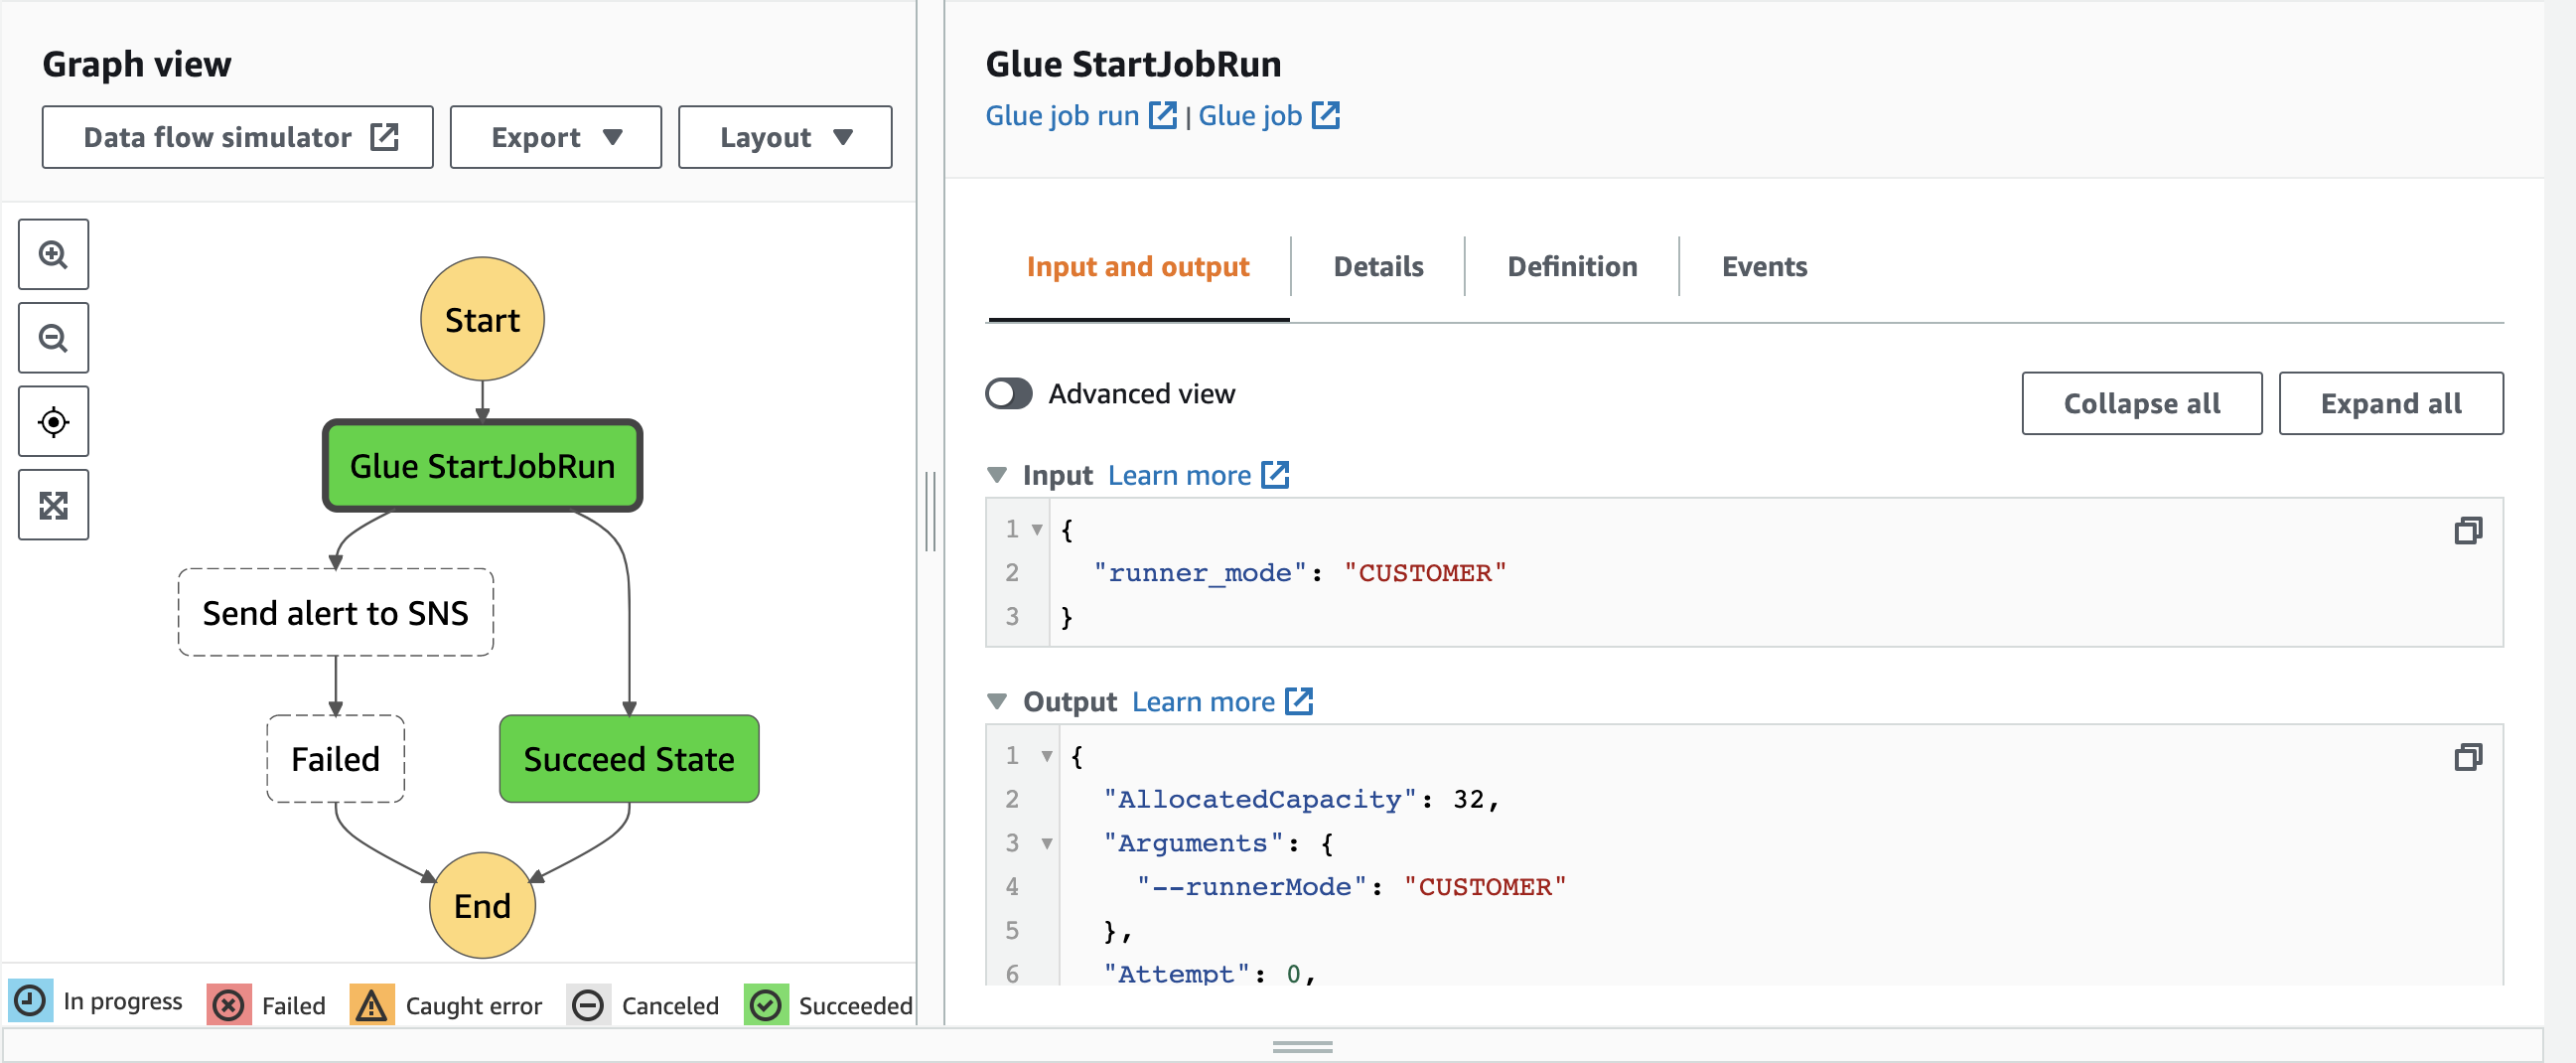
\includegraphics[width=\textwidth]{img/step-function-example.png}
        \centering
        \caption{Esempio di \textit{Step Function} che esegue un job Glue con diversi parametri.}
        \label{fig:step-function-example}
    \end{figure}
    \item \textbf{SecretsManager} - \textit{Amazon Secrets Manager} permette di modificare periodicamente, gestire e recuperare credenziali di database, chiavi API e altre chiavi segrete in tutto il loro ciclo di vita~\cite{aws-secrets-manager}.
    \item \textbf{Athena} - \textit{Amazon Athena} è un servizio di analisi interattivo serverless basato su framework open source, che supporta formati di file e tabelle aperte.
    Fornisce un modo semplificato e flessibile per analizzare petabyte di dati dove risiede.
    Permette di analizzare i dati o creare applicazioni da bucket Amazon Simple Storage Service (S3) e oltre 25 origini dei dati, incluse origini dei dati on-premise o altri sistemi cloud utilizzando SQL o Python.
    Athena è basato su motori \textit{Trino} e \textit{Presto} open source e framework Apache Spark, senza necessità di provisioning o configurazione~\cite{aws-athena}.
    \item \textbf{OpenSearch} - Consiste in una suite di analisi dei dati e ricerca distribuita, controllata dalla community, con licenza Apache 2.0 e open source utilizzata per un'ampia gamma di casi d'uso come il monitoraggio delle applicazioni in tempo reale e l'analisi dei dati di registro.
    OpenSearch fornisce un sistema altamente scalabile per fornire accesso e risposta rapidi a grandi volumi di dati con uno strumento di visualizzazione integrato, \textit{OpenSearch Dashboards}, che semplifica l'esplorazione dei dati da parte degli utenti.
    Si basa sulla libreria di ricerca Apache Lucene e supporta una serie di funzionalità di ricerca e analisi dei dati come la ricerca \textit{k-nearest neighbors} (KNN), SQL, Anomaly Detection, Machine Learning Commons, Trace Analytics, la ricerca full-text e altro ancora~\cite{aws-open-search}.
\end{itemize}
Il principale svantaggio di \textit{IaaS} e \textit{PaaS}, e in generale di tutte le tecnologie \textit{as a Service}, è il rischio di \textbf{lock in}.
I fornitori come \textit{Amazon} offrono un servizio che obbliga i fruitori ad adoperare tecnologie specifiche.
Sebbene sia un vantaggio per chi offre i servizi, questo potrebbe invece risultare problematico per chi li compra.
La scelta di un \textit{service provider} in fase di progettazione potrebbe causare danni economici anche notevoli in fase di sviluppo nel caso in cui questo non soddisfi a pieno le aspettative del fruitore.
Da ciò si deduce quanto sia importante essere in grado di migrare da un \textit{cloud provider} a un altro;
questa possibilità dipende fortemente dalla portabilità delle applicazioni sviluppate e dei dati mantenuti in \textit{cloud}.

L'utilizzo di AWS come \textit{PaaS} permette di soddisfare il requisito principale del progetto, ovvero l'esecuzione di un ETL sulla base di dati ricevuti.
Come discusso nella sezione~\ref{sec:etl-architecture}, la ricezione di flussi può avvenire per intero o parzialmente, cioè storicizzati.
I servizi di AWS possono essere integrati tra di loro per customizzare la gestione differente di questi flussi:
ad esempio, si può configurare \textit{Glue} per eseguire l'ETL al caricamento di nuovi dati direttamente su \textit{S3}.

\begin{figure}
    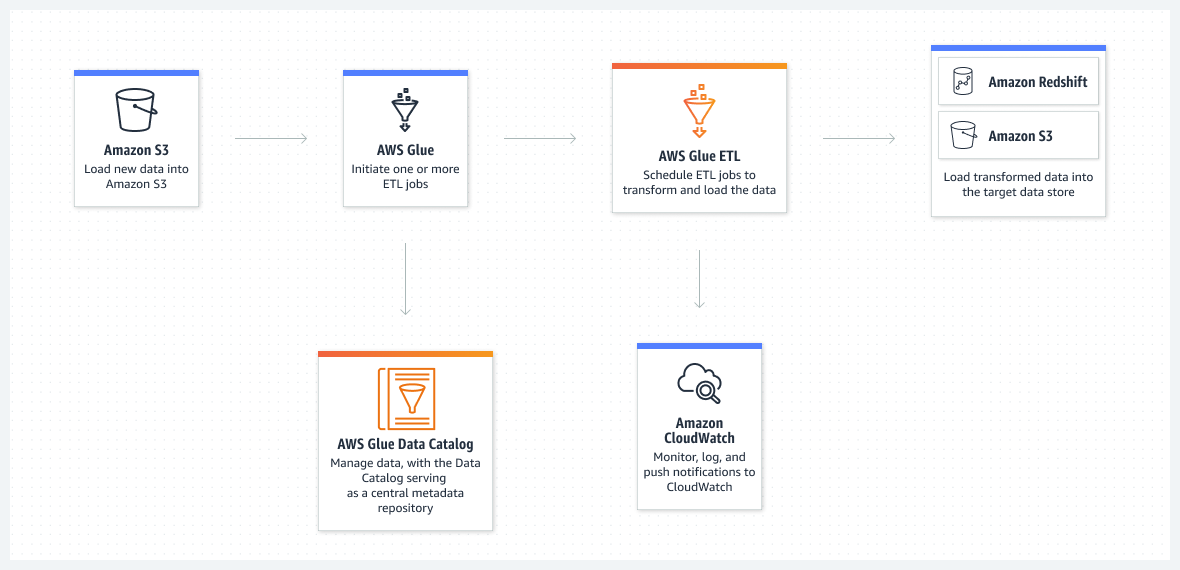
\includegraphics[width=\textwidth]{img/event-based-etl-on-glue.png}
    \centering
    \caption{Integrazione dei serivizi di AWS per realizzare un ETL basato su eventi~\cite{aws-glue}.}
    \label{fig:event-based-etl-on-glue}
\end{figure}
